\chapter{Related Work}

\section{Deep Learning and Supervised Learning}

Deep Learning (DL)~\cite{deeplearning} is a subclass of ML focused on algorithms inspired by the structure and function of the brain, known as artificial neural networks (NNs). Supervised Learning is an approach where the model learns from examples in the training set to generalize to new, unseen data and it forms the backbone of many ML applications, including DL.

\subsection{The Importance of Data Augmentation}

Data is a critical resource in ML and particularly in DL. However, collecting a large and diverse dataset is often impractical due to time, scale, financial, and other constraints. This is where data augmentation comes into play. Data augmentation is the process of artificially increasing the size and diversity of a dataset, traditionally by applying various transformations like rotation, scaling, and flipping to the existing data or more complex techniques like the ones this work focuses on. Research from Luis Perez et al.~\cite{perez} gives a good comparison among older and newer techniques, proposing a method based on NNs to choose the best one for a given classifier. 

\section{Generative Models}

Generative models~\cite{GenerativeModel} are a class of statistical models that aim to learn the underlying data distribution of the training set so that new data points can be generated. They have been successfully employed in various applications, including but not limited to, image synthesis and text generation. In the current work, they will be utilized for data augmentation.

\subsection{Generative Adversarial Networks}

Generative Adversarial Networks (GANs)~\cite{goodfellow} are a specialized form of DL models designed for generating synthetic yet realistic data. A GAN comprises two neural networks: the Generator (\(G\)) and the Discriminator (\(D\)). These networks are trained in tandem, engaging in a zero-sum game where the Generator aims to produce data indistinguishable from real data, and the Discriminator strives to distinguish between real and generated data.

\textbf{Architecture:} The Generator network takes a random noise vector \(z\) as input and produces synthetic data \(G(z)\). The Discriminator network takes both real data \(x\) and generated data \(G(z)\) as input and outputs a probability score indicating the likelihood that the data is real. A schematic representation of this architecture can be seen in Figure~\ref{fig:gan_training_process}.

\textbf{Loss Function:} The training process involves optimizing specific loss functions for both networks. The Discriminator aims to maximize the following loss function:
\[
\text{Discriminator Loss} = -\log(D(x)) - \log(1 - D(G(z)))
\]
Conversely, the Generator tries to minimize:
\[
\text{Generator Loss} = -\log(D(G(z)))
\]

\begin{figure}[H]
\centering
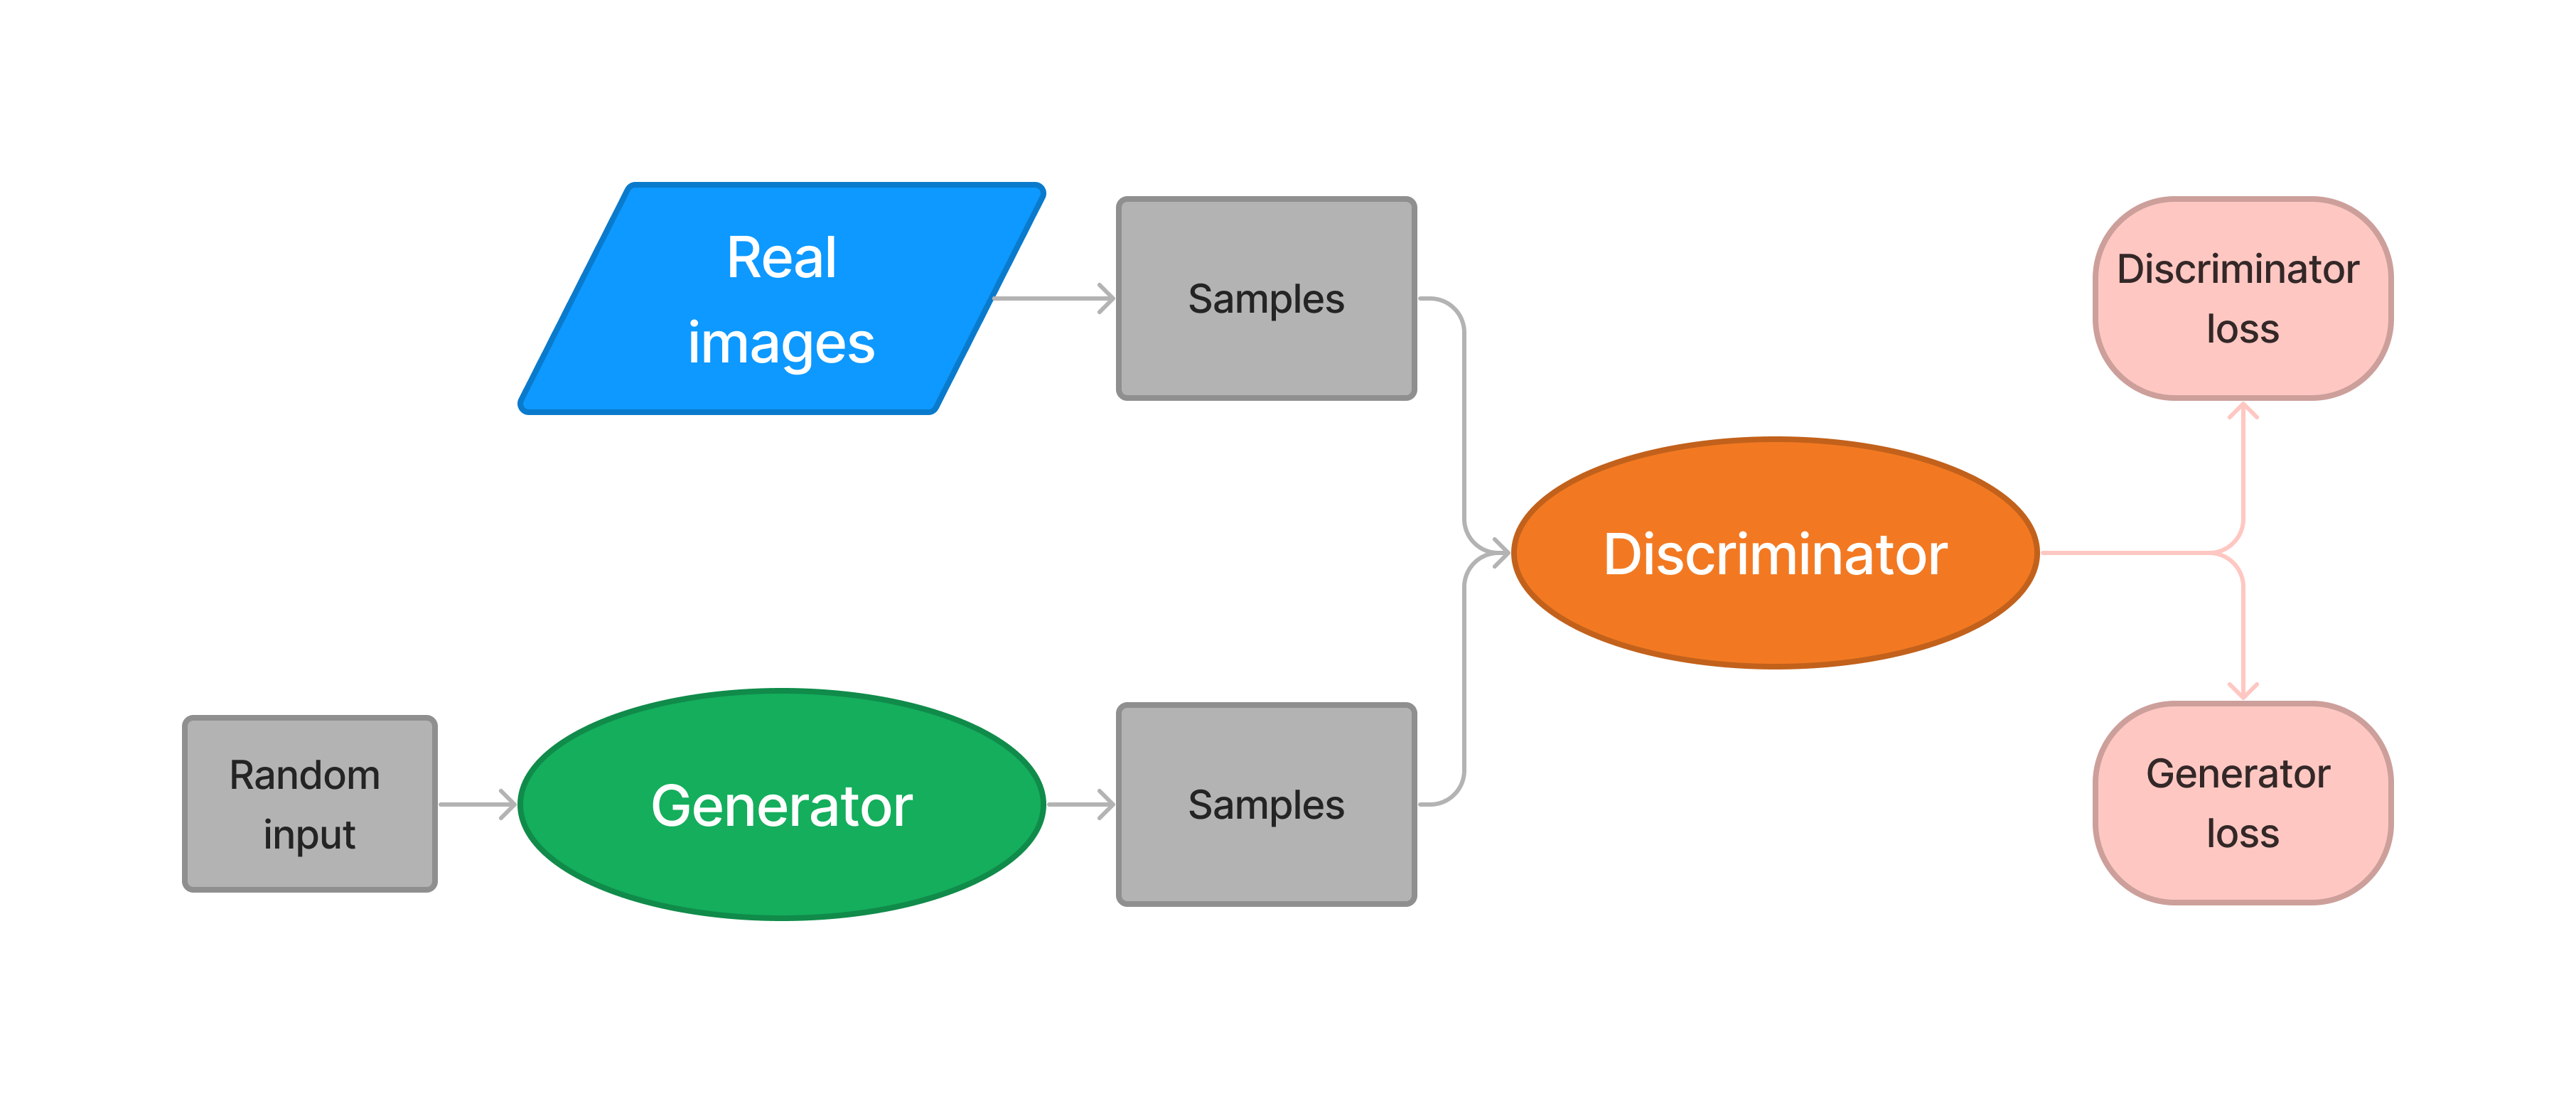
\includegraphics[width=\columnwidth]{main/content/images/diagrams/GAN.png}
\caption{Schematic representation of the GANs training process}
\label{fig:gan_training_process}
\end{figure}

\textbf{Applications in Data Augmentation:} GANs have proven effective in enhancing dataset diversity and improving model performance across various tasks~\cite{goodfellow, shorten}. For instance, Sundaram and Hulkund (2021) utilized GANs for data augmentation on the CheXpert chest X-ray dataset. Their study revealed that GAN-based augmentation significantly improved performance in underrepresented classes, particularly when data is scarce, thereby highlighting the promise of GANs in scenarios where data collection is expensive or impractical~\cite{sundaram}.

        
\subsection{Diffusion Models}

Diffusion models (DMs)~\cite{DDPM} are deep generative models that work by adding noise (Gaussian noise) to the available training data (the forward diffusion process) and then reversing the process (the denoising or the reverse diffusion process) to recover the data. 

\textbf{Training Process:} During the forward diffusion process, Gaussian noise is added to each layer of the neural network, corrupting the data gradually. The reverse diffusion process aims to recover the original data from the noise. This is achieved by minimizing a specific loss function that measures the difference between the original and the recovered data. A visual diagram of this architecture is illustrated in Figure~\ref{fig:dm_training_process}

\begin{figure}[H]
\centering
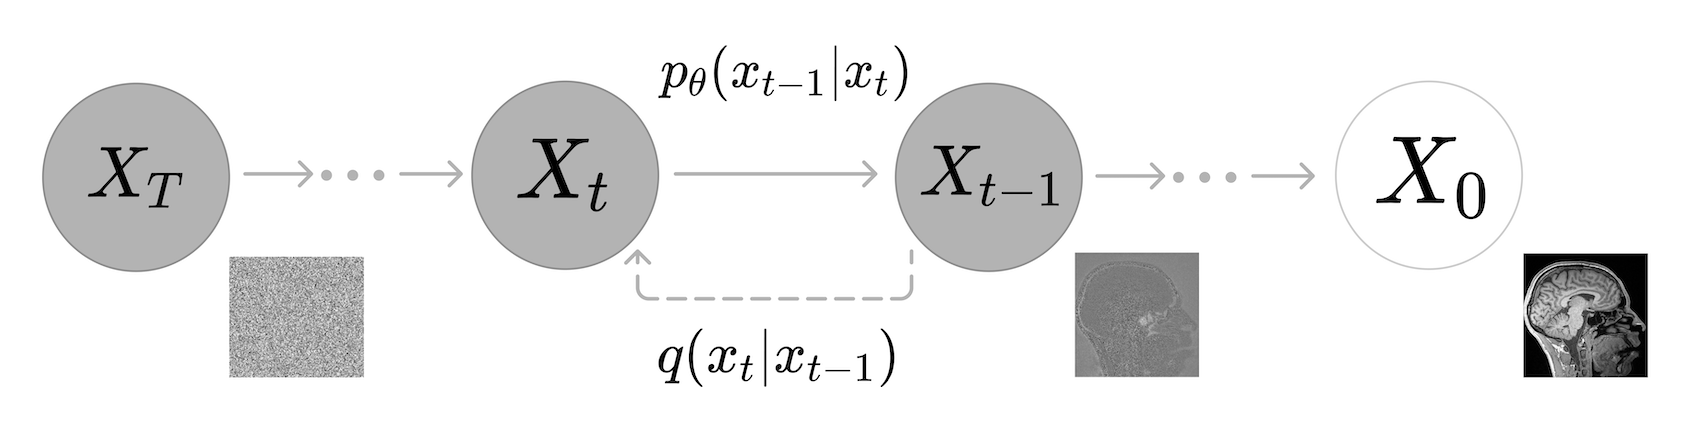
\includegraphics[width=\columnwidth]{main/content/images/diagrams/dm.png}
\caption{Schematic representation of the DMs training process.}
\label{fig:dm_training_process}
\end{figure}

DMs have been successfully applied to a variety of image generation tasks, including processing, colorization, super-resolution, inpainting, and semantic editing (Ruifei et al.~\cite{he2023synthetic}, Trabucco et al.~\cite{trabucco2023effective}, Azizi et al.~\cite{azizi2023synthetic}).

In particular, diffusion models have been used to generate large-scale images from text descriptions. A few notable examples, some of them with different versions, include:
    \begin{itemize}
        \item \textit{Stable Diffusion}~\cite{stable_diffusion}.
        \item \textit{DALL-E 2}~\cite{dalle2}.
        \item \textit{Imagen}~\cite{imagen}.
        \item \textit{eDiff}~\cite{balaji2023ediffi}.
        \item \textit{GLIDE}~\cite{glide}.
        \item \textit{Midjourney}~\cite{midjourney}.
        \item CM3leon~\cite{cm3leon}
    \end{itemize}
These models have produced incredible and high-resolution synthetic images.

Recently, DMs have been used to augment training data, for instance, synthetic data generated with GLIDE has been shown to improve the performance of zero-shot and few-shot image classification~\cite{he2023synthetic}. Other studies have explored strategies for augmenting individual images using pretrained DMs, with promising results in few-shot settings~\cite{trabucco2023effective}. During the course of our work, Azizi et al.~\cite{azizi2023synthetic} demonstrated that the \textit{Imagen} model can be fine-tuned for ImageNet~\cite{deng2009imagenet} to produce class-conditional models, achieving SOTA results.

However, images and domain-specific language in the medical field differ from natural images and texts, which can make it challenging for text-to-image models to generalize well into this domain. In the same direction, Chambon et al.~\cite{chambon2022roentgen} adapted a pretrained DM to a corpus of chest X-rays and their respective radiology reports. The resulting RoentGen model is proficient at generating high-fidelity, diverse synthetic medical images that are controllable via text prompts. In a similar vein to our work, RoentGen model has also been employed for data augmentation, leading to enhanced classifier performance. Nevertheless, the computational overhead for these advancements is substantial, RoentGen required the use of 64 A100 GPUs. This makes the approach less accessible and commercially viable for broader applications. To quantify this, we consider the cost of running such experiments on Google Cloud~\cite{cloudgpusCloudGPUs} , known for its cost-effective A100 GPU rates at \$1.25 per hour:

\begin{itemize}
    \item Fine-tuning a model for 1,000 training steps incurs an approximate cost of \$26.67.
    \item Extending the training to 12,500 steps raises the cost to around \$400.
    \item A full-scale training run of 60,000 steps would demand about \$1,920.
\end{itemize}

These estimates solely cover the GPU usage and do not account for other associated costs like storage, data transfer, or additional cloud services. Therefore, the actual expenditure could be significantly higher, further accentuating the computational and financial barriers for the adoption of such sophisticated models.
